
%%%%%%%%%%%%%%%%%%%%%%%%%%%%
%
% Accuracy vs Iterations: Normal Graph I
% Group the figures into one
\begin{figure*}[htbp]
	\centering
	\begin{subfigure}[b]{\textwidth}
		\centering
	% ???????????
	\begin{minipage}[b]{0.05\textwidth}
		\centering
        \raisebox{1.5cm}{
	\tiny % ????????????
	\renewcommand{\baselinestretch}{0.8}\selectfont % ?????
	\begin{tabular}{c}
		F \\
		A \\
		C \\
		E \\
		B  \\
		O \\
		O \\
		K
	\end{tabular}
	}
		%\raisebox{1.5cm}{\rotatebox{90}{\textbf{Main Title}}} % ?????????
	\end{minipage}%
	% ?????
	\begin{minipage}[b]{0.3\textwidth}
		\centering
		\caption*{Global Error} % ???
		\includegraphics[width=\textwidth]{images/facebook/figures_normal/Absolute_Error_vs_T.png} % ?????????
		
	\end{minipage}%
	% ?????
	\begin{minipage}[b]{0.3\textwidth}
		\centering
		\caption*{Local Error} % ???
		\includegraphics[width=\textwidth]{images/facebook/figures_normal/Multiplicative_Error_vs_T.png} % ?????????
		
	\end{minipage}%
	% ?????
	\begin{minipage}[b]{0.3\textwidth}
		\centering
		\caption*{Number of Inversions} % ???
		\includegraphics[width=\textwidth]{images/facebook/figures_normal/inv_vs_T.png} % ?????????
	\end{minipage}
\end{subfigure}

%%%%%%%%%%
%%%%%%%%%
\caption{Approximation Quality vs Number of Iterations: Selected Normal Graphs}
\label{fig:accuracy_iteration_normal_1}
\end{figure*}




%%%%%%%%%%%%%%%%%%%%%%%%%%%%%%
%%%%%%%%%%%%%%%%%%%%%%%%%%%%%

\begin{figure*}[htbp]
\centering
\begin{subfigure}[b]{\textwidth}
	\centering
\begin{minipage}[b]{0.3\textwidth}
			\centering
			%\caption*{Time-Normal Graph} % ???
			\includegraphics[width=\textwidth]{images/time_mem/time_normal/time_comparison_table.png} % ?????????
			
		\end{minipage}%
		% ?????
		\begin{minipage}[b]{0.3\textwidth}
			\centering
			%\caption*{Memory-Normal Graph} % ???
			\includegraphics[width=\textwidth]{images/time_mem/mem_normal/memory_usage_table.png} % ?????????
			
		\end{minipage}%

		\caption{Running Time and Memory Usage vs Graph Size on Normal Graphs}
\label{fig:time_mem_normal}
\end{subfigure}
\begin{subfigure}[b]{\textwidth}
	\centering
	\begin{minipage}[b]{0.3\textwidth}
	\centering
	%\caption*{Time-Hyper Graph} % ???
	\includegraphics[width=\textwidth]{images/time_mem/time_hyper/time_comparison_table.png} % ?????????
	
\end{minipage}%
% ?????
\begin{minipage}[b]{0.3\textwidth}
	\centering
	%\caption*{Memory-Hyper Graph} % ???
	\includegraphics[width=\textwidth]{images/time_mem/mem_hyper/memory_usage_table.png} % ?????????
\end{minipage}%
	\caption{Running Time and Memory Usage vs Graph Size on Double Covers}
\label{fig:time_mem_double}
\end{subfigure}
\caption{}
\label{fig:time_mem}
\end{figure*}



%%%%%%%%%%%%%
%
%  Simulated Wall Clock Time
% Group the figures into one
\begin{figure*}[htbp]
	\centering
	\begin{subfigure}[b]{\textwidth}
		\centering
		% ???????????
		\begin{minipage}[b]{0.05\textwidth}
			\centering
			\raisebox{1.5cm}{
				\tiny % ????????????
				\renewcommand{\baselinestretch}{0.8}\selectfont % ?????
				\begin{tabular}{c}
					F \\
					A \\
					C \\
					E \\
					B  \\
					O \\
					O \\
					K
				\end{tabular}
			}
			%\raisebox{1.5cm}{\rotatebox{90}{\textbf{Main Title}}} % ?????????
		\end{minipage}%
		% ?????
		\begin{minipage}[b]{0.3\textwidth}
			\centering
			\caption*{Global Error} % ???
			\includegraphics[width=\textwidth]{images/facebook/figures_normal/Absolute_Error_vs_Time.png} % ?????????
			
		\end{minipage}%
		% ?????
		\begin{minipage}[b]{0.3\textwidth}
			\centering
			\includegraphics[width=\textwidth]{images/facebook/figures_normal/Multiplicative_Error_vs_Time.png} % ?????????
			
		\end{minipage}%
		% ?????
		\begin{minipage}[b]{0.3\textwidth}
			\centering
			\caption*{Number of Inversions} % ???
			\includegraphics[width=\textwidth]{images/facebook/figures_normal/inv_vs_Time.png} % ?????????
		\end{minipage}
	\end{subfigure}
	%%
	\caption{Approximation Quality vs Simulated Wall Clock Time: Selected Normal Graphs}
	\label{fig:accuracy_time_normal_graphs_1}
\end{figure*}

%%%%%%%%%%%%%%%%%%%%%%%%%%%
% Group the figures into one


\begin{figure*}[bp]
	%\begin{figure*}[H]
	\centering
	\begin{subfigure}[b]{\textwidth}
		\centering
		% ???????????
		\begin{minipage}[b]{0.05\textwidth}
			\centering
			\raisebox{1.5cm}{
				\tiny % ????????????
				\renewcommand{\baselinestretch}{0.8}\selectfont % ?????
				\begin{tabular}{c}
					F \\
					A \\
					C \\
					E \\
					B \\
					O \\
					O \\
					K
				\end{tabular}
			}
			%\raisebox{1.5cm}{\rotatebox{90}{\textbf{Main Title}}} % ?????????
		\end{minipage}%
		% ?????
		\begin{minipage}[b]{0.3\textwidth}
			\centering
			\includegraphics[width=\textwidth]{images/parameters/facebook/figures/Absolute_Error_vs_T.png} % ?????????
			
		\end{minipage}%
		% ?????
		\begin{minipage}[b]{0.3\textwidth}
			\centering
			
			\includegraphics[width=\textwidth]{images/parameters/facebook/figures/Multiplicative_Error_vs_T.png} % ?????????
			
		\end{minipage}%
		% ?????
		\begin{minipage}[b]{0.3\textwidth}
			\centering
			
			\includegraphics[width=\textwidth]{images/parameters/facebook/figures/inv_vs_T.png} % ?????????
		\end{minipage}
	\end{subfigure}
	%%%%%
	\caption{Approximation Quality vs Number of Iterations for \prexp with Different $C$ in 
		$\gamma_t = 1 - \frac{C}{t+C}$, for $C = 1, 2, \ldots, 6$
	}
	\label{fig:parameter_normal_graphs}
\end{figure*}




%%%%%%%%%%%%%
%%%%%%%%%%%%


% Group the figures into one
\begin{figure*}[htbp]
	\centering

		\begin{subfigure}[b]{\textwidth}
			\centering
			% ???????????
			\begin{minipage}[b]{0.05\textwidth}
				\centering
				\raisebox{1.5cm}{
					\tiny % ????????????
					\renewcommand{\baselinestretch}{0.8}\selectfont % ?????
					\begin{tabular}{c}
						F \\
						A \\
						C \\
						E \\
						B  \\
						O \\
						O \\
						K
					\end{tabular}
				}
				%\raisebox{1.5cm}{\rotatebox{90}{\textbf{Main Title}}} % ?????????
			\end{minipage}%
			% ?????
			\begin{minipage}[b]{0.3\textwidth}
				\centering
				\caption*{Global Error} % ???
				\includegraphics[width=\textwidth]{images/facebook/figures_hyper/Absolute_Error_vs_T.png} % ?????????
				
			\end{minipage}%
			% ?????
			\begin{minipage}[b]{0.3\textwidth}
				\centering
				\caption*{Local Error} % ???
				\includegraphics[width=\textwidth]{images/facebook/figures_hyper/Multiplicative_Error_vs_T.png} % ?????????
				
			\end{minipage}%
			% ?????
			\begin{minipage}[b]{0.3\textwidth}
				\centering
				\caption*{Number of Inversions} % ???
				\includegraphics[width=\textwidth]{images/facebook/figures_hyper/inv_vs_T.png} % ?????????
			\end{minipage}
		\end{subfigure}
	
	%
	\caption{Approximation Quality vs Number of Iterations: Selected Double Covers}
	\label{fig:errors_hyper}
\end{figure*}







% Group the figures into one
\begin{figure*}[htbp]
	\centering

		\begin{subfigure}[b]{\textwidth}
			\centering
			% ???????????
			\begin{minipage}[b]{0.05\textwidth}
				\centering
				\raisebox{1.5cm}{
					\tiny % ????????????
					\renewcommand{\baselinestretch}{0.8}\selectfont % ?????
					\begin{tabular}{c}
						F \\
						A \\
						C \\
						E \\
						B  \\
						O \\
						O \\
						K
					\end{tabular}
				}
				%\raisebox{1.5cm}{\rotatebox{90}{\textbf{Main Title}}} % ?????????
			\end{minipage}%
			% ?????
			\begin{minipage}[b]{0.3\textwidth}
				\centering
				\caption*{Global Error} % ???
				\includegraphics[width=\textwidth]{images/facebook/figures_hyper/Absolute_Error_vs_Time.png} % ?????????
				
			\end{minipage}%
			% ?????
			\begin{minipage}[b]{0.3\textwidth}
				\centering
				\caption*{Local Error} % ???
				\includegraphics[width=\textwidth]{images/facebook/figures_hyper/Multiplicative_Error_vs_Time.png} % ?????????
				
			\end{minipage}%
			% ?????
			\begin{minipage}[b]{0.3\textwidth}
				\centering
				\caption*{Number of Inversions} % ???
				\includegraphics[width=\textwidth]{images/facebook/figures_hyper/inv_vs_Time.png} % ?????????
			\end{minipage}
		\end{subfigure}
	%
	\caption{Approximation Quality vs Simulated Wall Clock Time: Selected Double Covers}
	\label{fig:errors_hyper_time}
\end{figure*}